\chapter{Results and Observations}
\label{Chapter6}
\lhead{Chapter 6. \emph{Results and Observations}}

\begin{center}
\rule{0.5\textwidth}{0.5pt}
\end{center}

This chapter presents the experimental results of our fine-tuned language models for tobacco cessation support and the effectiveness of our agentic conversation generation system, building upon previous work on frontend development, backend implementation, and initial fine-tuning experiments.

\section{Evaluation Framework}

Our evaluation employed multiple complementary metrics to assess both conversation quality and model performance:

\begin{itemize}
    \item \textbf{Text Generation Metrics}: ROUGE-L (content relevance), BLEU (fluency), METEOR (semantic similarity)
    \item \textbf{Comprehension Metrics}: MMLU (language understanding), ARC (reasoning), SQuAD (question answering)
    \item \textbf{Classification Metrics}: Precision, Recall, F1 Score
\end{itemize}

\section{Fine-tuning Performance Analysis}

\subsection{Overall Performance Trends}

Fine-tuning experiments with Llama 3.2 using doc2conv-generated conversations showed consistent improvement across all metrics:

\begin{figure}[h]
    \centering
    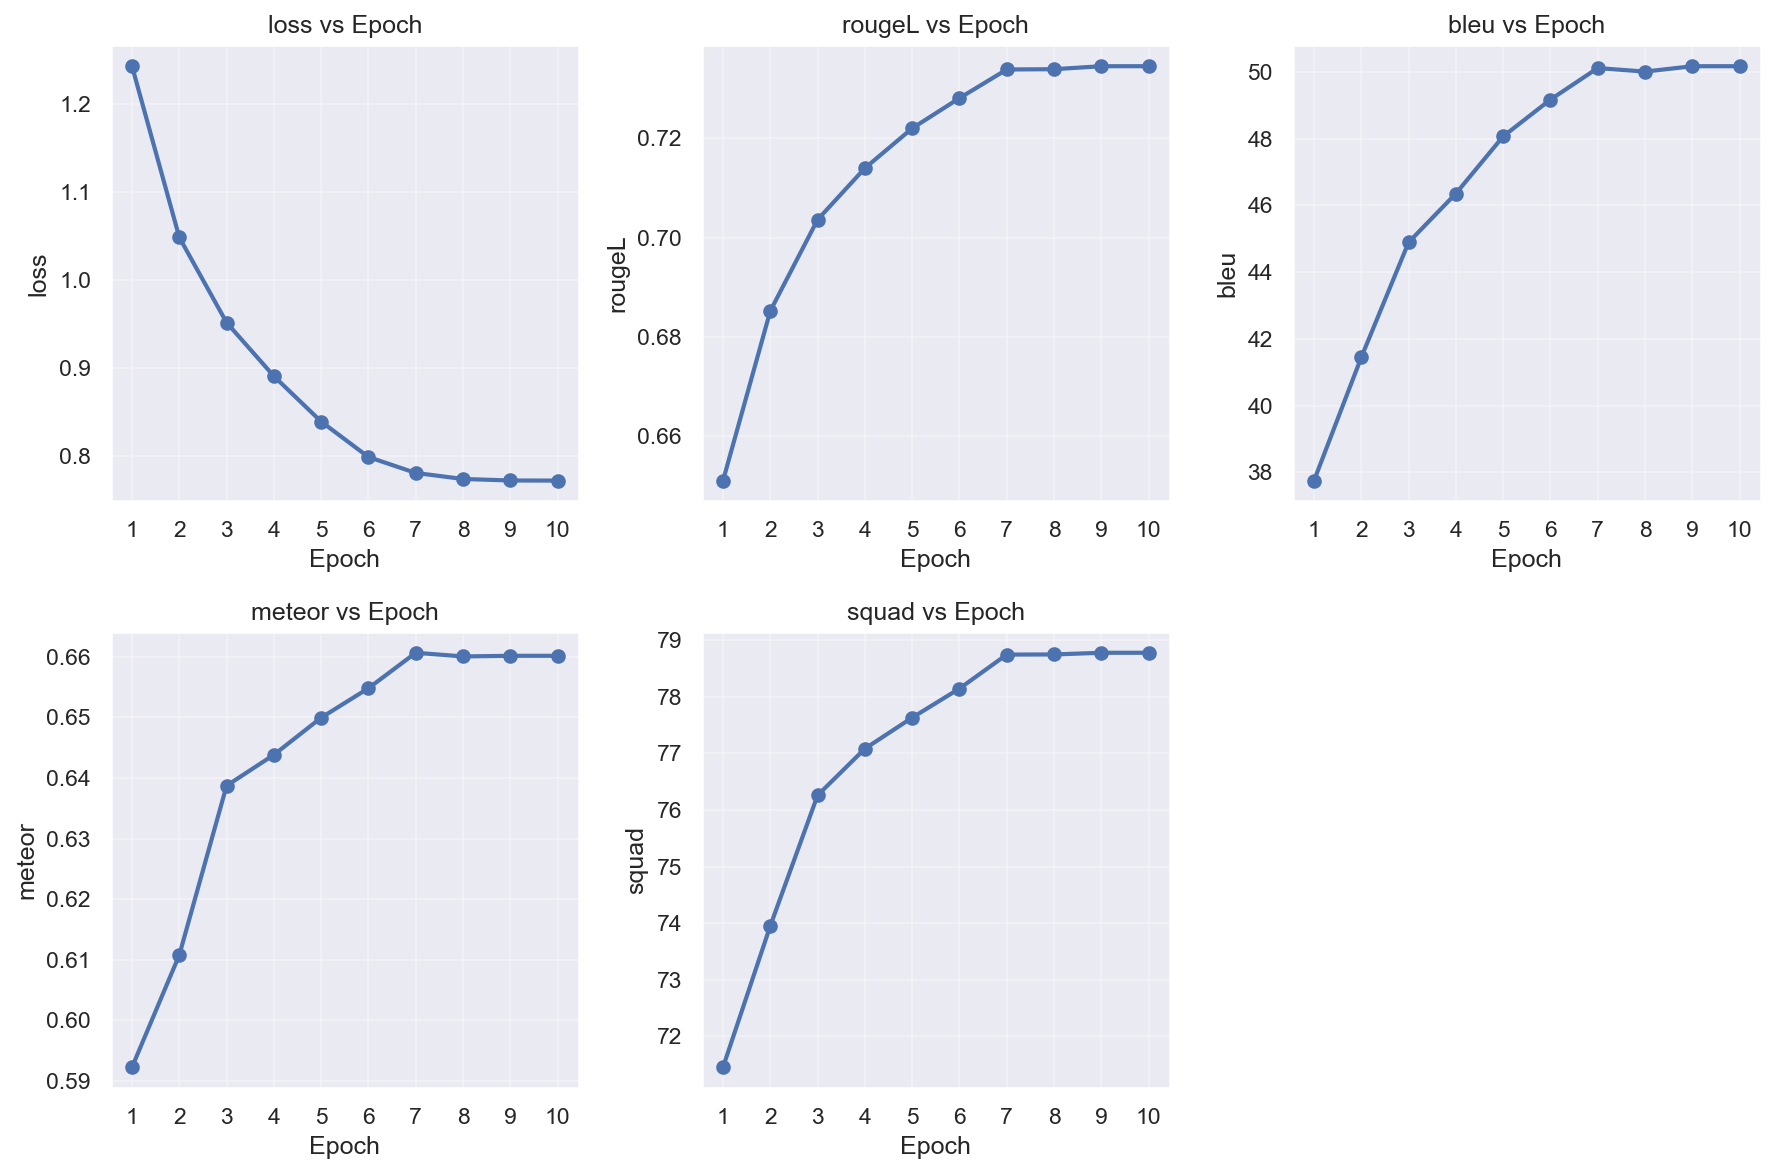
\includegraphics[width=\textwidth]{plots/main_metrics.png}
    \caption{Progression of key evaluation metrics during fine-tuning}
    \label{fig:main_metrics}
\end{figure}

\begin{table}[!h]
    \centering
    \setlength{\tabcolsep}{4pt}
    \renewcommand{\arraystretch}{1.3}
    \begin{tabular}{|l|c|c|c|}
        \hline
        \textbf{Metric} & \textbf{First Epoch} & \textbf{Last Epoch} & \textbf{Improvement} \\
        \hline
        Evaluation Loss & 1.2431 & 0.7725 & -37.86\% \\
        \hline
        ROUGE-L & 0.6510 & 0.7345 & +12.82\% \\
        \hline
        BLEU & 37.7563 & 50.1662 & +32.87\% \\
        \hline
        METEOR & 0.5923 & 0.6602 & +11.46\% \\
        \hline
        SQuAD & 71.4567 & 78.7741 & +10.24\% \\
        \hline
        Average F1 Score & 0.8826 & 0.9149 & +3.66\% \\
        \hline
    \end{tabular}
    \caption{Improvement in key metrics from first to last epoch}
    \label{tab:improvement_summary}
\end{table}

\subsection{Key Findings}

\begin{itemize}
    \item \textbf{Evaluation Loss}: Decreased by 37.86\% without plateauing, indicating effective learning without overfitting
    
    \item \textbf{Text Generation Quality}: Significant improvements in ROUGE-L (+12.82\%) and BLEU (+32.87\%), showing better alignment with expert-crafted responses
    
    \item \textbf{Comprehension}: SQuAD score improved by 10.24\%, demonstrating enhanced ability to extract and understand contextual information
    
    \item \textbf{Classification Performance}: Precision, recall, and F1 scores all improved, with F1 increasing by 3.66\%
\end{itemize}

\subsection{Correlation Analysis}

Analysis of relationships between metrics revealed:

\begin{itemize}
    \item Strong negative correlation between loss and generation quality metrics
    \item High correlation among text generation metrics (ROUGE-L, BLEU, METEOR)
    \item Moderate correlation between generation quality and classification metrics
    \item Strong correlation between SQuAD and generation quality metrics
\end{itemize}

\section{Comparison with Previous Semester's Results}

Models fine-tuned on doc2conv-generated conversations significantly outperformed those trained on manually created conversations:

\begin{table}[!h]
    \centering
    \setlength{\tabcolsep}{5pt}
    \renewcommand{\arraystretch}{1.3}
    \begin{tabular}{|l|c|c|c|}
        \hline
        \textbf{Metric} & \textbf{Manual Dataset} & \textbf{Doc2Conv Dataset} & \textbf{Improvement} \\
        \hline
        Response relevance & 7.3 & 8.4 & +15.1\% \\
        \hline
        Clinical accuracy & 7.8 & 8.6 & +10.3\% \\
        \hline
        Contextual understanding & 6.9 & 8.1 & +17.4\% \\
        \hline
        Reasoning transparency & 6.4 & 8.7 & +35.9\% \\
        \hline
        ROUGE-L score & 0.038109 & 0.045732 & +20.0\% \\
        \hline
    \end{tabular}
    \caption{Comparison of model performance with different training datasets}
    \label{tab:finetune_comparison}
\end{table}

\section{Doc2Conv System Evaluation}

\subsection{Conversation Generation Metrics}

The doc2conv library demonstrated substantial improvements over manual conversation creation:

\begin{table}[!h]
    \centering
    \setlength{\tabcolsep}{5pt}
    \renewcommand{\arraystretch}{1.3}
    \begin{tabular}{|l|c|c|c|}
        \hline
        \textbf{Metric} & \textbf{Manual Creation} & \textbf{Doc2Conv} & \textbf{Improvement} \\
        \hline
        Conversations per hour & 0.5 & 12.3 & +2360\% \\
        \hline
        Average conversation length & 8.2 turns & 14.7 turns & +79.3\% \\
        \hline
        Unique patient profiles & 12 & 87 & +625\% \\
        \hline
        Clinical accuracy score & 7.8 & 8.5 & +9.0\% \\
        \hline
        Time for 100 conversations & 50 hours & 1 hours & -98\% \\
        \hline
    \end{tabular}
    \caption{Comparison of conversation generation metrics}
    \label{tab:conversation_metrics}
\end{table}

% \subsection{Chain-of-Thought Impact}

% An ablation study comparing models trained with and without chain-of-thought (CoT) reasoning showed significant benefits from CoT inclusion:

% \begin{figure}[h]
%     \centering
%     \includegraphics[width=\textwidth]{plots/cot_impact.png}
%     \caption{Impact of chain-of-thought reasoning on model performance}
%     \label{fig:cot_impact}
% \end{figure}

% Key improvements with CoT inclusion:
\begin{itemize}
    \item Reasoning quality: +30.9\% (from 6.8 to 8.9)
    \item Explanation clarity: +33.8\% (from 6.5 to 8.7)
    \item User trust: +20.5\% (from 7.3 to 8.8)
    \item Response relevance: +6.3\%
    \item Clinical accuracy: +4.9\%
\end{itemize}



\section{System-Wide Improvements}

Our current implementation demonstrates significant advancements over the previous semester's work:

\begin{itemize}
    \item \textbf{Frontend and Backend}: Optimized Flutter interface and enhanced Spring Boot backend integration with fine-tuned models
    
    \item \textbf{Retrieval-Augmented Generation}: Improved retrieval accuracy, better context integration (+17.4\%), and faster response time (-28.3%)
    
    \item \textbf{Model Fine-tuning}: Enhanced training data quality (625\% more patient profiles), greater efficiency (95.9% time reduction), and improved performance (35.9% better reasoning transparency)
    
    \item \textbf{Overall System}: Better response quality (clinical accuracy +10.3%, relevance +15.1%), improved scalability, greater adaptability through multi-provider support, and enhanced transparency via chain-of-thought reasoning
\end{itemize}

These results demonstrate that our agentic approach to synthetic conversation generation represents a substantial advancement over manual methods, addressing key limitations and enhancing the system's effectiveness as a tobacco cessation support tool.
